\documentclass[12pt]{article}
\usepackage[utf8]{inputenc}
\usepackage{listings}
\usepackage{xcolor}
\usepackage{graphicx}
\definecolor{codegreen}{rgb}{0,0.6,0}
\definecolor{codegray}{rgb}{0.5,0.5,0.5}
\definecolor{codepurple}{rgb}{0.58,0,0.82}
\definecolor{backcolour}{rgb}{0.95,0.95,0.92}
\lstdefinestyle{mystyle}{
    backgroundcolor=\color{backcolour},   
    commentstyle=\color{codegreen},
    keywordstyle=\color{magenta},
    numberstyle=\tiny\color{codegray},
    stringstyle=\color{codepurple},
    basicstyle=\ttfamily\footnotesize,
    breakatwhitespace=false,         
    breaklines=true,                 
    captionpos=b,                    
    keepspaces=true,                 
    numbers=left,                    
    numbersep=5pt,                  
    showspaces=false,                
    showstringspaces=false,
    showtabs=false,                  
    tabsize=2
}

\lstset{style=mystyle}
\begin{document}
\title{CSDS 391 Programming Assignment 2 Writeup}
\author{Ningjia Huang, Tianxi Zhao}
\date{Due On: December 4, 2020}
\maketitle

\section*{Problem 1: }

\section*{Problem 2: }
\subsection*{(a)}
The mean squared error is calculated using the following equation: 
\begin{center}
    $MSE = \frac{1}{n}\sum_n (Y_i - \hat{Y_i})^2$
\end{center}
, where $Y_i$ is the actual category of the $ith$ item and $\hat{Y_i}$ is the predicted category by using our neural network.\\ \\
The following codes compute the \textbf{mean squared error} for iris data. The parameter "data\_vector" are the attributes we would like to take into account, it should be a dataframe of attributes.
$w_0, w_1, w_2$ define the weights of neural network. The parameter "pattern\_classes" is a dataframe of the category corresponding to the data\_vectors. The \textbf{mean\_square\_error} makes use of 
the logistic non-linearity function in Problem 1.
\begin{lstlisting}[language=Python, caption=Mean Squared Error Calculation]
# data vectors in dataframe, pattern classes in list
def mean_square_error(data_vectors, w0, w1, w2, pattern_classes):
    n = data_vectors.shape[0]
    data_vectors_list = data_vectors.values.tolist()
    pattern_classes_list = pattern_classes.tolist()
    temp_mse = 0
    for i in range(n):
        temp_mse = temp_mse + np.square(pattern_classes_list[i] - one_layer_network(w0, w1, w2, data_vectors_list[i][0], data_vectors_list[i][1]))
    mse = temp_mse/n
    return mse
\end{lstlisting}

\subsection*{(b)}
To plot the linear boundary, we find the x-intercept and y-intercept by using the following code: 
\begin{lstlisting}
plot([0,-w0/w1],[-w0/w2,0])
\end{lstlisting}
\subsubsection*{2.b.1}
The first set of weights we've chosen is $[-3.9, 0.46, 0.95]$. The mean squared error we concluded is 0.05. The following figure shows the linear boundary with our chosen set of weights. As we can tell from the graph, the
linear boundary generally seperates the two categories of iris. 
\begin{center}
    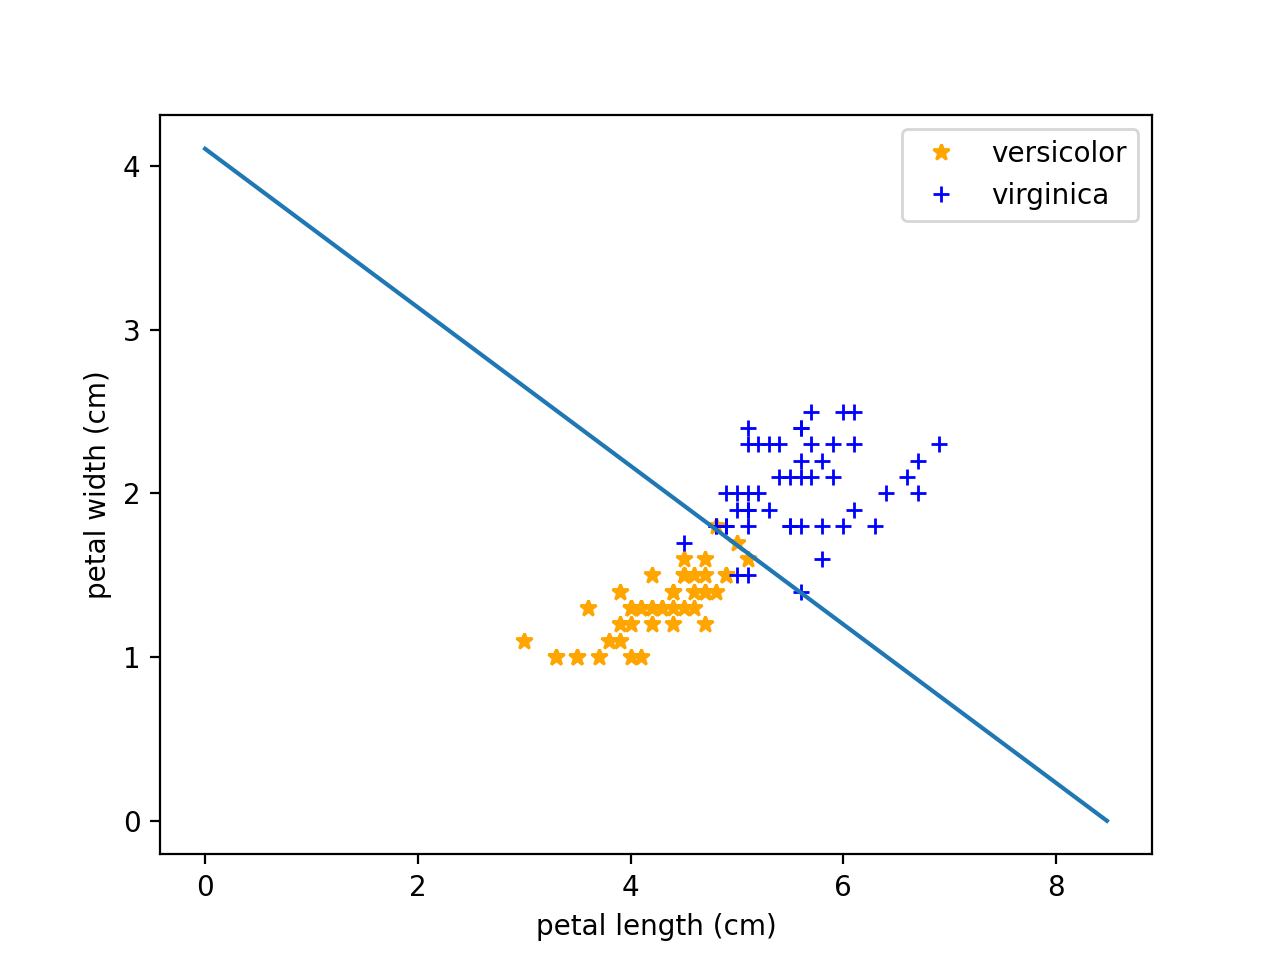
\includegraphics[scale=0.6]{fig/p2_b1.png}
\end{center}

\subsubsection*{2.b.2}
The second set of weights we've chosen is $[-1, 0.7, 2]$. The mean squared error we concluded is 0.5. The following figure shows the linear boundary with our chosen set of weights. As we can tell from the graph, the linear boundary does not seperate these two categories 
at all. 
\begin{center}
    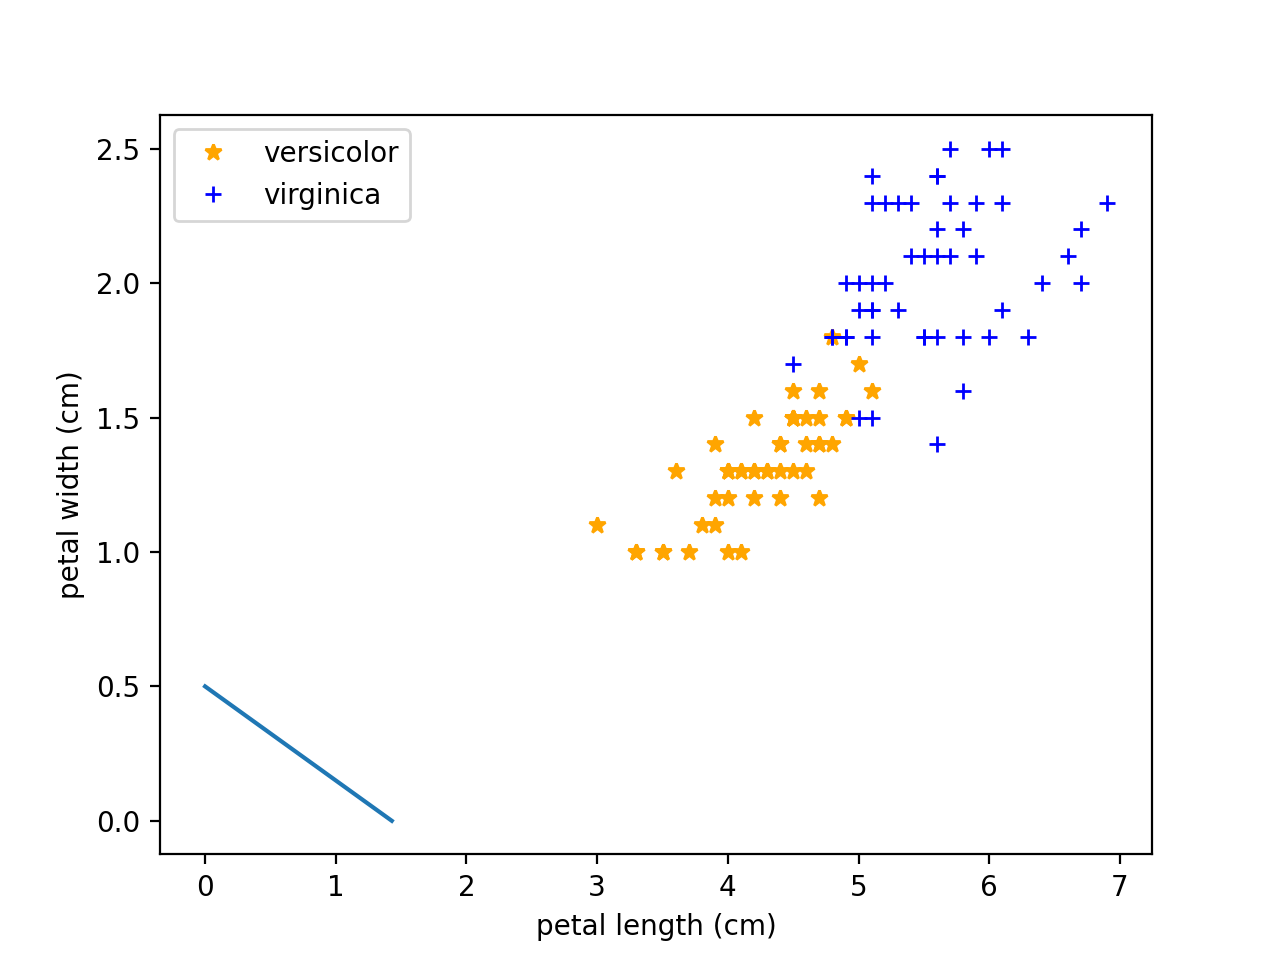
\includegraphics[scale=0.6]{fig/p2_b2.png}
\end{center}

\subsection*{(c)}
To compute the gradient of the objective function, we need to take the derivative of the objective function. Assume \textbf{x$_i$} is the ith row with attribute petal length and petal width such that $x_i = [1,x_{i1},x_{i2}]$($1$ is placed here because $w_0$ requires 1 to be its coefficient). \textbf{w} is the set of weights for the attributes. The logistic function we get is:
\begin{center}
    $\sigma(z) = \frac{1}{1+e^{-z}} = \frac{1}{1+e^{w \cdot x}}$
\end{center}
Therefore, the mean squared function becomes: 
\begin{center}
    $MSE = \frac{1}{N} \sum_{i = 1}^{n}(\sigma(w\cdot x_i)-y_i)^2$
\end{center}
By taking the derivative of this objective function with respect to $w_0$, we have: 
\begin{center}
    $\frac{\partial MSE}{\partial w_0} = \frac{2}{N}\sum_{i=1}^{N}(\sigma(w \cdot x_i)-y_i)\frac{\partial \sigma}{\partial w_0}$ \\ 
    $\frac{\partial MSE}{\partial w_0} = \frac{2}{N}\sum_{i=1}^{N}(\sigma(w \cdot x_i)-y_i)(1-\sigma(w \cdot x_i))(\sigma(w\cdot x_i))\frac{\partial (w\cdot x)}{\partial w_0}$ \\ 
    $\frac{\partial MSE}{\partial w_0} = \frac{2}{N}\sum_{i=1}^{N}(\sigma(w \cdot x_i)-y_i)(1-\sigma(w \cdot x_i))(\sigma(w\cdot x_i))$
\end{center}
Similarly, by only changing the last derivative $\frac{\partial(w\cdot x)}{\partial w_0}$ to $\frac{\partial(w\cdot x)}{\partial w_1}$ and $\frac{\partial(w\cdot x)}{\partial w_2}$, we can compute the derivative of the objective function with respect to $w_1$ and $w_2$:
\begin{center}
    $\frac{\partial MSE}{\partial w_1} = \frac{2}{N}\sum_{i=1}^{N}(\sigma(w \cdot x_i)-y_i)(1-\sigma(w \cdot x_i))(\sigma(w\cdot x_i))x_{i1}$
    $\frac{\partial MSE}{\partial w_2} = \frac{2}{N}\sum_{i=1}^{N}(\sigma(w \cdot x_i)-y_i)(1-\sigma(w \cdot x_i))(\sigma(w\cdot x_i))x_{i2}$
\end{center} 

\subsection*{(d)}
\end{document}